
%
%	Sketches for Q9(b)(v)
%
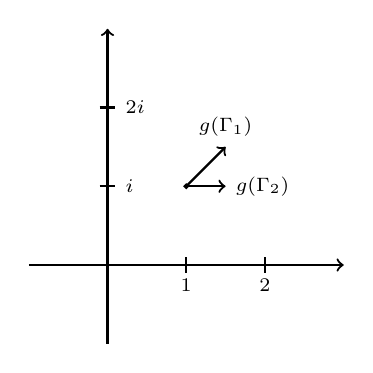
\begin{tikzpicture}
	% grid for draft only
	%%\draw [help lines] (-1,-1) grid (3,3);
	% the X-axis
	\draw[->,thick] (-1,0)--(3,0);
	\draw[thick] (1,-0.1) -- (1,0.1) node[below=4pt] {\scriptsize $1$};
	\draw[thick] (2,-0.1) -- (2,0.1) node[below=4pt] {\scriptsize $2$};
	% the Y-axis
	\draw[->,thick] (0,-1)--(0,3);
	\draw[thick] (-0.1,1) -- (0.1,1) node[right] {\scriptsize $i$};
	\draw[thick] (-0.1,2) -- (0.1,2) node[right] {\scriptsize $2i$};
	% little dot at g(1)
	\draw[thick] (1,1) circle(0.02);
	% g(\Gamma_1)
	\draw[->,thick] (1,1) -- (1.5,1.5) node[above] {\scriptsize $g(\Gamma_1)$};
	% g(\Gamma_2)
	\draw[->,thick] (1,1) -- (1.5,1) node[right] {\scriptsize $g(\Gamma_2)$};
\end{tikzpicture}

